\chapter*{\textbf{Capítulo IV: Análisis de Resultados}}
\label{ch:Resultados}
\addcontentsline{toc}{chapter}{\textbf{IV. Análisis de Resultados}}
\chead{Análisis de Resultados}
\setcounter{chapter}{4}
\setcounter{equation}{0}
\setcounter{figure}{0}
\setcounter{table}{0}

\section*{IV.1 Simulaciones}
\addcontentsline{toc}{section}{IV.1 Simulaciones}

Primeramente se presentan los resultados de las metodologías para la mejora de la SNR en las curvas simuladas.

\subsection*{IV.1.1 Mejora de la señal a ruido en curvas de luz}
\addcontentsline{toc}{subsection}{IV.1.1 Mejora de la señal a ruido en curvas de luz}

Con el propósito de evaluar estadísticamente el desempeño de la metodología planteada en este trabajo, se combinaron las bases de datos de ruidos simulados (véase III.2.3) y de tránsitos simulados (véase III.3) para una prueba de ajuste del modelo del trapezoide y probar el criterio de validación de tránsitos. Se insertaron los tránsitos simulados a las curvas de ruido para distintos valores de señal a ruido (SNR). Las 625 curvas de tránsitos, con cada una de las 100 curvas de ruido. Esto genera un total de 62,500 pruebas por valor de SNR, y un total de 2,500 pruebas por valor de $\Delta F$.

Esto nos genera una distribución 2500 SNR's por cada valor de $\Delta F$, para resumir este resultado, presentamos el intervalo que contiene el 90\% de los resultados, excluyendo los casos más extremos. Es decir, cada intervalo de las tablas \ref{tab_mejora_snr_10} y \ref{tab_mejora_snr_100} está compuesto por el percentil 5, 50 y 95.  

\begin{table}[H]
	\centering
	\begin{tabular}{ccccccccc}
	\hline 
	$\Delta F$ & $\mbox{SNR}_{Fourier}$ &  $\mbox{SNR}_{mov}$ & $\mbox{SNR}_{PCA}$\\ 
	\hline
	0.03 & 	${56.12}_{-22.53}^{+21.43}$ & ${46.39}_{-17.83}^{+26.5}$ & ${66.95}_{-22.37}^{+20.83}$ \\
	0.02 &  ${65.82}_{-29.63}^{+42.01}$ & ${51.0}_{-21.18}^{+50.29}$ & ${86.41}_{-37.71}^{+38.48}$ \\
	0.01 & ${73.24}_{-36.93}^{+96.5}$ & ${55.08}_{-24.24}^{+86.07}$ & ${112.47}_{-58.77}^{+91.6}$ \\
	0.002 & ${76.25}_{-38.76}^{+163.78}$ & ${56.83}_{-25.37}^{+108.36}$	& ${127.94}_{-69.19}^{+228.57}$ \\
	\hline 
	\end{tabular} 
	\caption{Resultados de la mejora de la SNR para tránsitos simulados, a los cuales se les insertó un ruido simulado de $SNR=10$. $\Delta F$ representa la variación en el flujo de la estrella debido al tránsito. $\mbox{SNR}_{Fourier}$, $\mbox{SNR}_{mov}$ y $\mbox{SNR}_{PCA}$ indican el valor de SNR de la curva de luz, obtenida mediante el filtrado de Fourier, promedio móvil y PCA respectivamente. Los intervalos del 90\% fueron obtenidos a partir de la distribución de SNR's que resultan de las pruebas, con $N=2500$ casos únicos para cada $\Delta F$.}
	\label{tab_mejora_snr_10}
	\end{table}


\begin{table}[H]
	\centering
	\begin{tabular}{ccccccccc}
	\hline 
	$\Delta F$ & $\mbox{SNR}_{Fourier}$ &  $\mbox{SNR}_{mov}$ & $\mbox{SNR}_{PCA}$\\ 
	\hline
	0.03 & 	${81.71}_{-4.37}^{+4.01}$ & ${80.91}_{-4.74}^{+3.74}$ & ${81.22}_{-3.82}^{+4.11}$ \\
	0.02 &  ${123.01}_{-10.47}^{+7.08}$ & ${120.85}_{-12.16}^{+7.21}$ & ${123.04}_{-8.96}^{+7.65}$ \\
	0.01 & ${240.81}_{-47.93}^{+24.17}$ & ${226.68}_{-47.63}^{+32.63}$ & ${248.12}_{-36.71}^{+27.47}$ \\
	0.002 & ${548.05}_{-237.59}^{+474.3}$ & ${439.0}_{-182.87}^{+497.27}$ & ${784.99}_{-357.55}^{+456.92}$ \\
	\hline 
	\end{tabular} 
	\caption{Resultados de la mejora de la SNR para tránsitos simulados, a los cuales se les insertó un ruido simulado de $SNR=100$. $\Delta F$ representa la variación en el flujo de la estrella debido al tránsito. $\mbox{SNR}_{Fourier}$, $\mbox{SNR}_{mov}$ y $\mbox{SNR}_{PCA}$ indican el valor de SNR de la curva de luz, obtenida mediante el filtrado de Fourier, promedio móvil y PCA respectivamente. Los intervalos del 90\% fueron obtenidos a partir de la distribución de SNR's que resultan de las pruebas, con $N=2500$ casos únicos para cada $\Delta F$.}
	\label{tab_mejora_snr_100}
	\end{table}

Como puede verse en las tablas \ref{tab_mejora_snr_10} y \ref{tab_mejora_snr_100}, el valor de la SNR depende de la variación en el flujo $\Delta F$, los tránsitos profundos disminuyen la SNR, sin embargo podemos apreciar que los valores centrales son comparables.

El análisis de componentes principales parece tener el mejor desempeño. Como se puede apreciar en la figura \ref{fig_transito_pca}, el resultado es una curva suave con SNR alta. Sin embargo en la misma imágen podemos apreciar la diferencia entre el modelo y la curva filtrada, por lo que la medida de la SNR, no nos sugiere cual es el mejor método.

Debido a esto, comparamos también las curvas resultantes del filtrado con el modelo trapezoidal, para evaluar el desempeño de las diferentes metodologías, los resultados se presentan a continuación.

\subsection*{IV.1.2 Determinación de candidatos a tránsitos}
\addcontentsline{toc}{subsection}{IV.1.2 Determinación de candidatos a tránsitos}

Para determinar la eficiencia de la metodología en la identificación de candidatos a tránsitos de exoplanetas, se utilizó el coeficiente de correlación como medida de la calidad del filtrado. Utilizando la base de datos de tránsitos simulados (véase III.3.1) y los ruidos simulados (véase III.2.3) se calcularon los coeficientes de correlación de 625 casos únicos (25 $\Delta F$ y 25 $t_{c}$), las mismas simulaciones que dieron lugar a los resultados presentados en la subsección anterior (IV.1.1).

Presentaremos los resultados por método de filtrado, y para los casos límites de ruido, es decir $SNR=10$ y $SNR=100$. Estos valores de SNR's son de antes de cualquier proceso de filtrado.

\subsubsection*{IV.1.2.1 Correlaciones resultantes del filtrado de Fourier}
\addcontentsline{toc}{subsubsection}{IV.1.2.1 Correlaciones resultantes del filtrado de Fourier}

Las figuras \ref{fig_correlaciones_fou_10} y \ref{fig_correlaciones_fou_100} muestran la correlación, entre el modelo y la curva filtrada con el filtro de Fourier, para curvas con $SNR=10$ y $SNR=100$ respectivamente. El color nos indica la media de los coeficientes de correlación ($C$), de los 100 ruidos con diferentes parámetros (véase III.2.3).

\begin{figure}[h!]
	\centering
		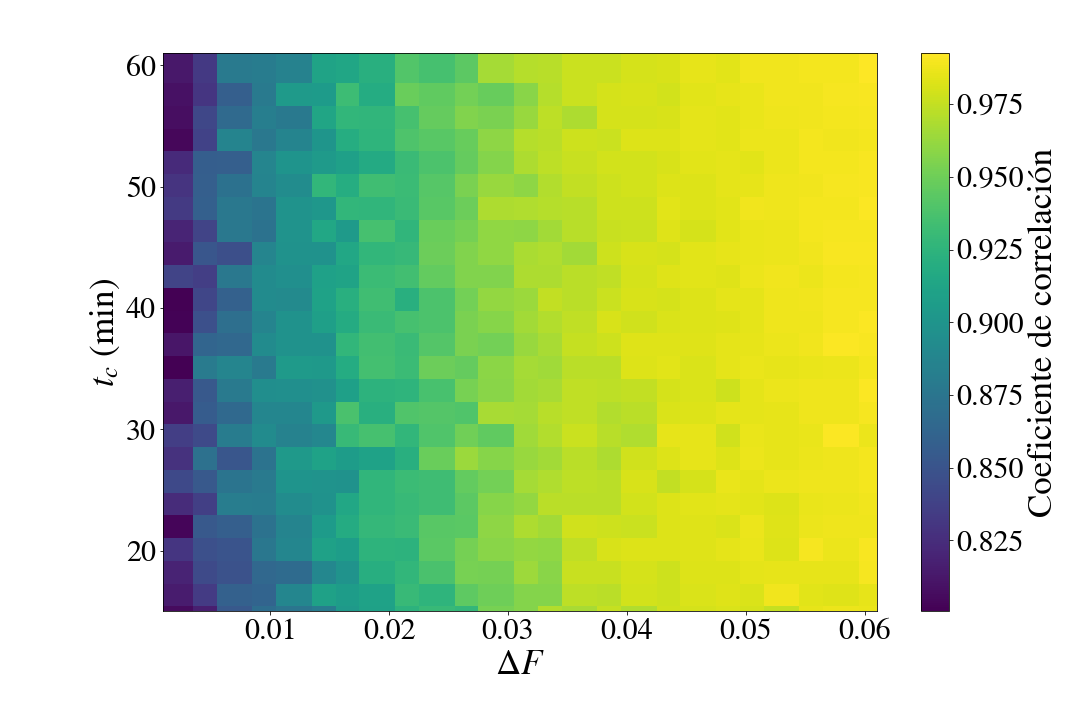
\includegraphics[max size={0.9\textwidth}{0.36\textheight}]{./figures/corrFourierSNR_10.png}
		\caption{Mapa de correlaciones de los parámetros $\Delta F$ y $t_{c}$ entre las simulaciones y los calculados después de aplicar el modelo del trapezoide a los datos filtrados utilizando Fourier. Estos resultados se obtuvieron a partir de curvas simuladas con una $SNR=10$.}
		\label{fig_correlaciones_fou_10}
\end{figure}

\begin{figure}[h!]
	\centering
		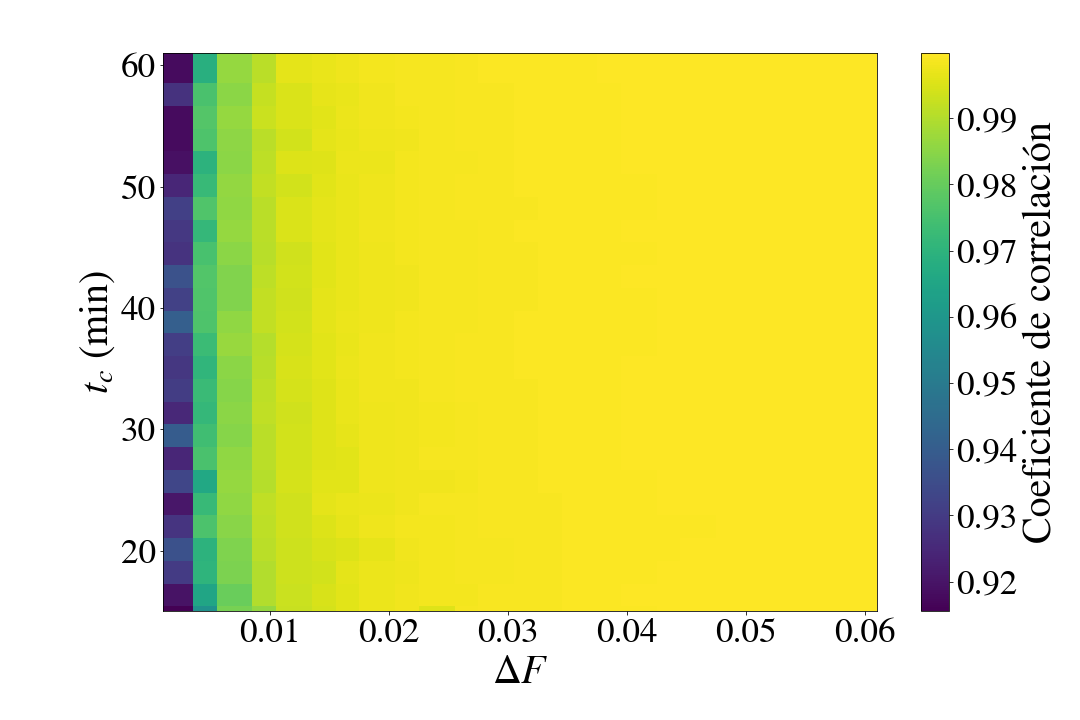
\includegraphics[max size={0.9\textwidth}{0.36\textheight}]{./figures/corrFourierSNR_100.png}
		\caption{Mapa de correlaciones de los parámetros $\Delta F$ y $t_{c}$ entre las simulaciones y los calculados después de aplicar el modelo del trapezoide a los datos filtrados utilizando Fourier. Estos resultados se obtuvieron a partir de curvas simuladas con una $SNR=100$.}
		\label{fig_correlaciones_fou_100}
\end{figure}

Estos resultados ayudan a saber que tipos de sistemas planetarios, podrían ser detectados utilizando esta metodología. También nos ayuda a definir la cota inferior para el coeficiente de correlación entre el modelo y la curva filtrada, para que esta, sea considerada como candidato a tránsito. Para el método de filtrado con Fourier, la cota inferior para el coeficiente de correlación es de $C \geq 0.85 $. 

Esta cota inferior se calculó a partir de un estudio de falsos positivos, donde se aplicó la metodología planteada en este trabajo, a curvas con solo ruido. De estos resultados, tomamos el coeficiente de correlación máximo $C_{max}$ y calculamos la cota inferior como: 

\begin{equation}
	C_{cota}= \dfrac{1+C_{max}}{2}
\end{equation}


Si analizamos la figura \ref{fig_correlaciones_fou_100}, vemos que para las curvas con $SNR=100$, todo el intervalo de valores de $\Delta F$ y $t_{c}$ (dentro de los límites, véase IV.2) tiene un valor de $C$ es mayor que la cota inferior. Esto significaría, que en principio seríamos capaces de detectarlos. Por otra parte, en la figura \ref{fig_correlaciones_fou_10}, vemos que para curvas con $SNR=10$ los tránsitos con $\Delta F < \sim 0.005$ no serían detectables.

\subsubsection*{IV.1.2.2 Correlaciones resultantes del promedio móvil}
\addcontentsline{toc}{subsubsection}{IV.1.2.2 Correlaciones resultantes del promedio móvil}

De manera análoga, las figuras \ref{fig_correlaciones_mov_10} y \ref{fig_correlaciones_mov_100} muestran la correlación, entre el modelo y la curva filtrada con el promedio móvil, para curvas con $SNR=10$ y $SNR=100$ respectivamente. El color nos indica la media de los coeficientes de correlación ($C$), de los 100 ruidos con diferentes parámetros (véase III.2.3).

\begin{figure}[h!]
	\centering
		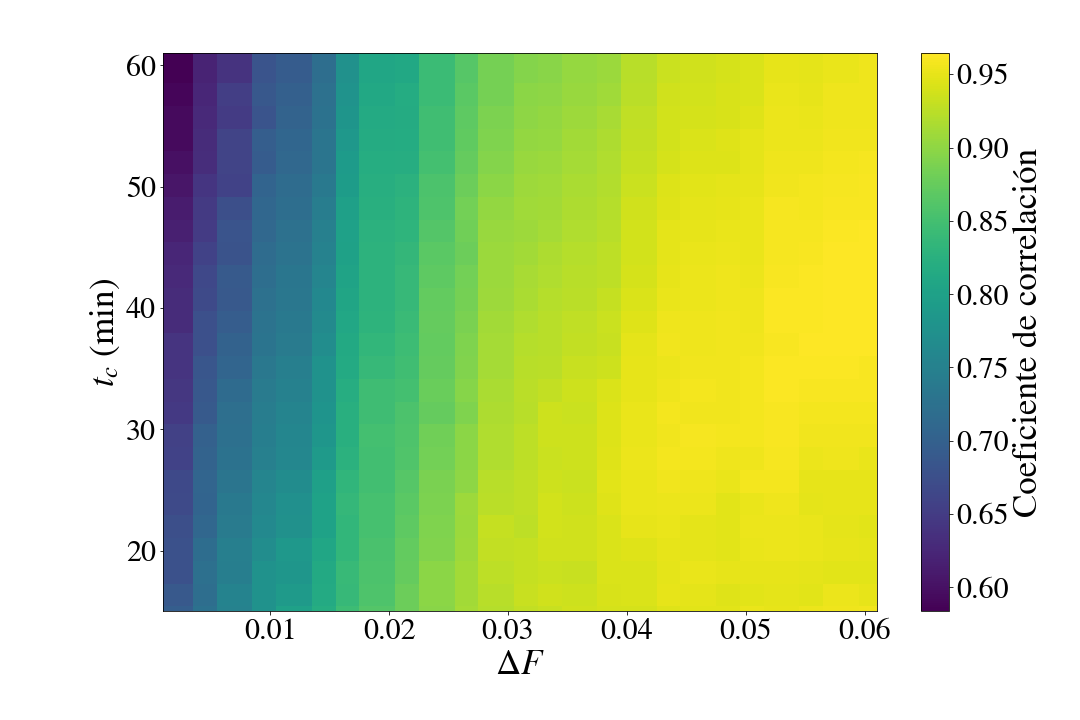
\includegraphics[max size={0.9\textwidth}{0.36\textheight}]{./figures/corrMovSNR_10.png}
		\caption{Mapa de correlaciones de los parámetros $\Delta F$ y $t_{c}$ entre las simulaciones y los calculados después de aplicar el modelo del trapezoide a los datos filtrados utilizando promedio móvil. Estos resultados se obtuvieron a partir de curvas con una $SNR=10$.}
		\label{fig_correlaciones_mov_10}
\end{figure}

\begin{figure}[h!]
	\centering
		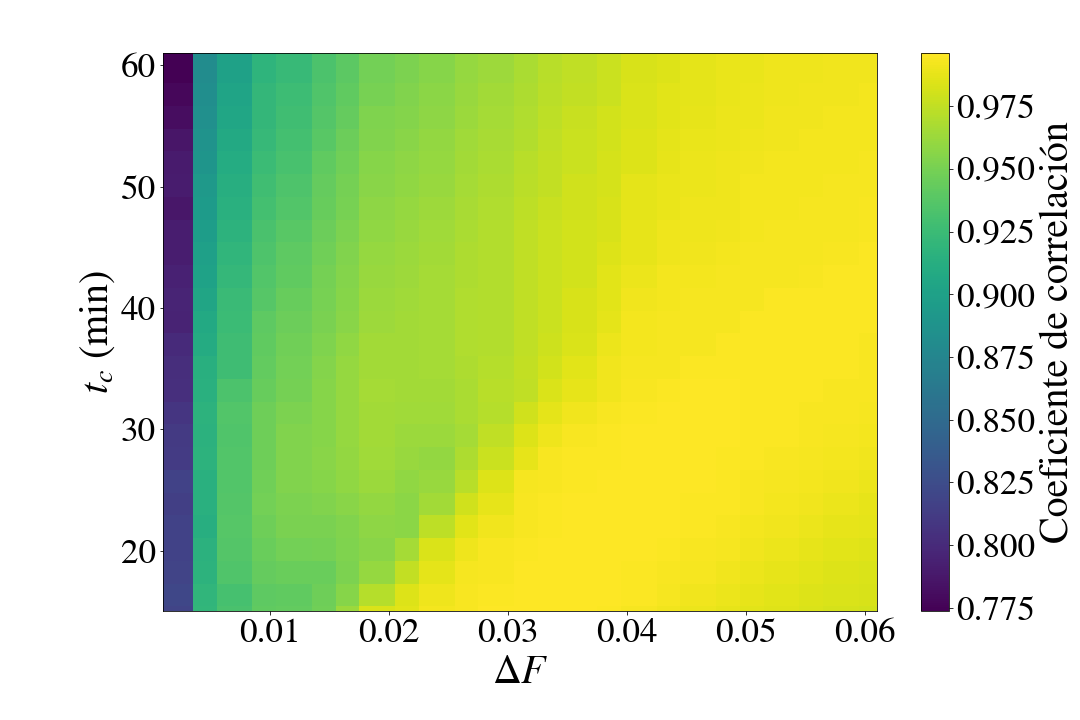
\includegraphics[max size={0.9\textwidth}{0.36\textheight}]{./figures/corrMovSNR_100.png}
		\caption{Mapa de correlaciones de los parámetros $\Delta F$ y $t_{c}$ entre las simulaciones y los calculados después de aplicar el modelo del trapezoide a los datos filtrados utilizando promedio móvil. Estos resultados se obtuvieron a partir de curvas con una $SNR=100$.}
		\label{fig_correlaciones_mov_100}
\end{figure}

Para el método de promedio móvil, la cota inferior para determinar una curva como candidata a tránsito es de $C \geq 0.84 $.

Si analizamos la figura \ref{fig_correlaciones_mov_100}, vemos que para este método de filtrado, los valores de $C$ están en función de $\Delta F$ y más notablemente de $t_{c}$. Esto se debe a lo que se mencionaba anteriormente (véase IV.1.2.2), este método altera la forma de la señal inmersa en el ruido. Esta deformación aumenta de manera proporcional a $t_{c}$.


\subsubsection*{IV.1.2.3 Correlaciones resultantes de PCA}
\addcontentsline{toc}{subsubsection}{IV.1.2.3 Correlaciones resultantes de PCA}

De manera análoga, las figuras \ref{fig_correlaciones_pca_10} y \ref{fig_correlaciones_pca_100} muestran la correlación, entre el modelo y la curva filtrada con el método de análisis de componentes principales (PCA), para curvas con $SNR=10$ y $SNR=100$ respectivamente. El color nos indica la media de los coeficientes de correlación ($C$), de los 100 ruidos con diferentes parámetros (véase III.2.3).

\begin{figure}[h!]
	\centering
		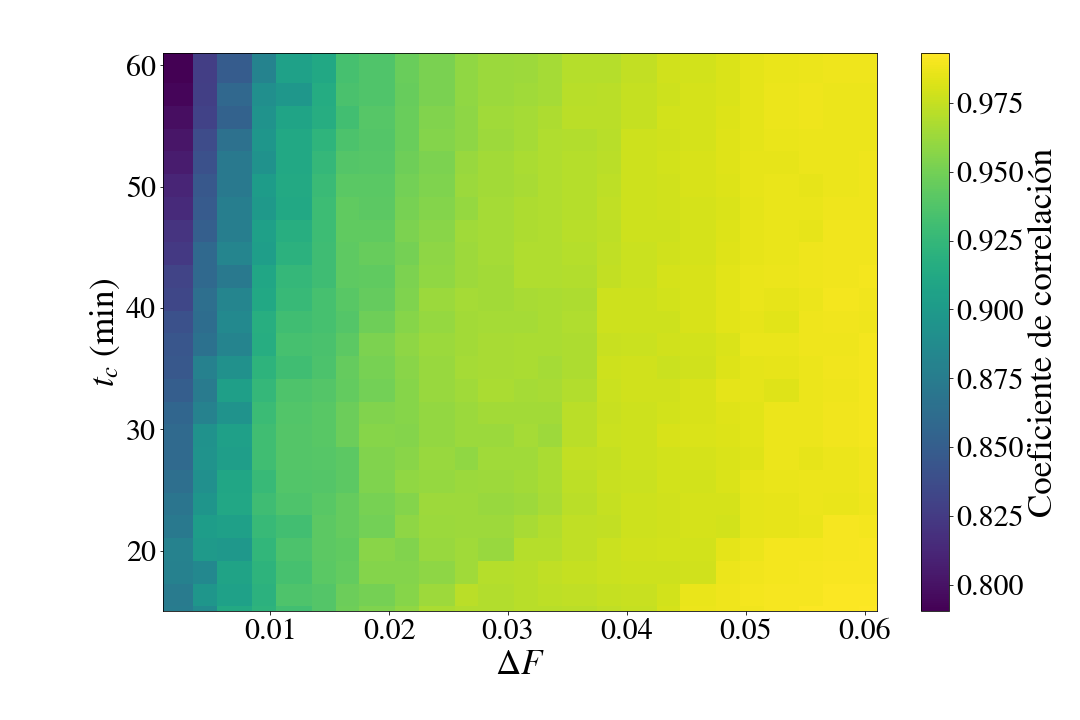
\includegraphics[max size={0.9\textwidth}{0.36\textheight}]{./figures/corrPCASNR_10.png}
		\caption{Mapa de correlaciones de los parámetros $\Delta F$ y $t_{c}$ entre las simulaciones y los calculados después de aplicar el modelo del trapezoide a los datos filtrados utilizando PCA. Estos resultados se obtuvieron a partir de curvas con una $SNR=10$.}
		\label{fig_correlaciones_pca_10}
\end{figure}

\begin{figure}[h!]
	\centering
		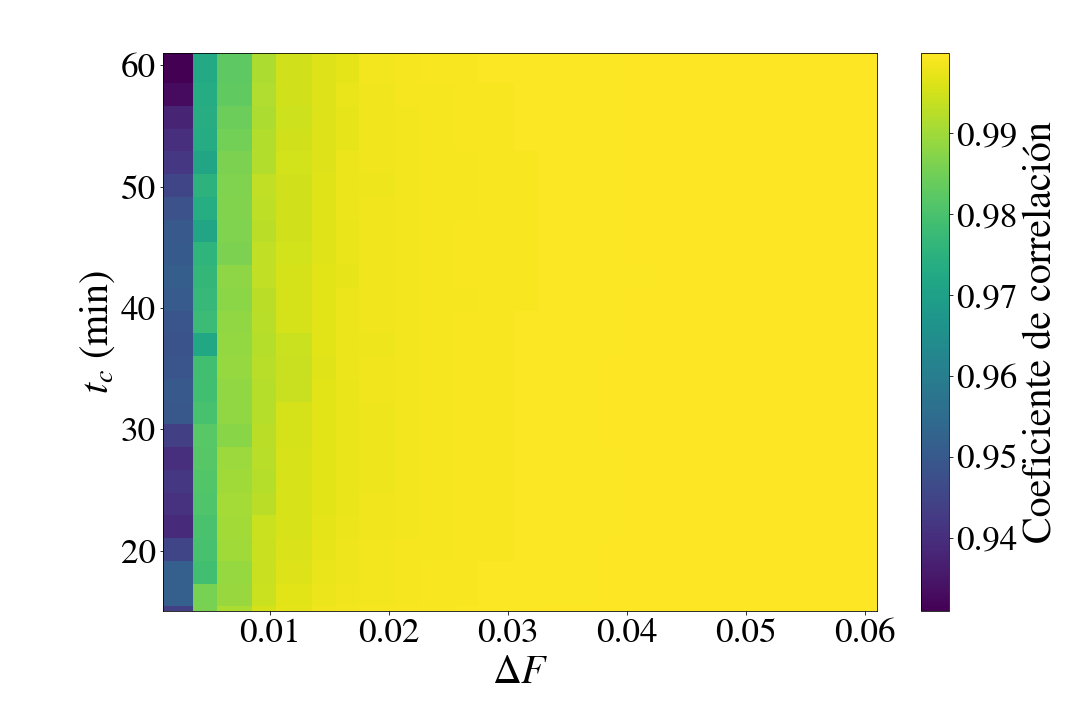
\includegraphics[max size={0.9\textwidth}{0.36\textheight}]{./figures/corrPCASNR_100.png}
		\caption{Mapa de correlaciones de los parámetros $\Delta F$ y $t_{c}$ entre las simulaciones y los calculados después de aplicar el modelo del trapezoide a los datos filtrados utilizando PCA. Estos resultados se obtuvieron a partir de curvas con una $SNR=100$.}
		\label{fig_correlaciones_pca_100}
\end{figure}

El filtrado usando PCA método arroja los coeficientes de correlación más altos, sin embargo lo mismo ocurrió en la prueba de falsos positivos. Para este método, la cota inferior para determinar una curva como candidata a tránsito es de $C \geq 0.94 $. 

Si analizamos las figuras  \ref{fig_correlaciones_pca_10} y \ref{fig_correlaciones_pca_100}, vemos que al igual que para el método de Fourier, no se ve una correlación significativa entre $C$ y $t_{c}$. 

\section*{IV.2 Datos observacionales}
\addcontentsline{toc}{section}{IV.2 Datos observacionales}

Se presentan los resultados de las metodologías para la mejora de la
SNR en las curvas de luz reales (véase III.1).

\subsection*{IV.2.1 Mejora de la señal a ruido en datos observacionales}
\addcontentsline{toc}{subsection}{IV.2.1 Mejora de la señal a ruido en datos observacionales}

Se presenta un ejemplo del resultado del filtrado de ruido en la curva de luz de alta cadencia de HAT-P-37b, utilizando las 3 metodologías descritas en la sección anterior: el filtro de frecuencias de Fourier, promedio móvil y análisis de componentes principales (PCA). La curva de luz de HAT-P-37b fue obtenida mediante fotometría de apertura, ya que no se encontraron estrellas de campo para la fotometría diferencial.

\begin{figure}[h!]
	\centering
	  \includegraphics[max size={0.9\textwidth}{0.9\textheight}]{./figures/hat37b_sinfil_2.png}
	 \caption{Curva de luz de HAT-P-37b tomada a 20 fps, durante la segunda mitad del tránsito. La curva de luz se obtuvo mediante fotometría de apertura con una $SNR=11.73$. La línea negra representa el modelo teórico, utilizando los parámetros presentados en \cite{bakos2012hat}.}
	  \label{fig_transito_hat37b}
  \end{figure}


\subsubsection*{IV.2.1.1 Resultados del filtro de Fourier}
\addcontentsline{toc}{subsubsection}{IV.2.1.1 Resultados del filtro de Fourier}

En la figura \ref{fig_transito_fou} podemos apreciar el resultado del filtro pasabajas de Fourier, aplicado a la curva de luz de HAT-P-37b. A pesar de ser una curva con mucho ruido, se puede apreciar a simple vista la forma del tránsito. Se utilizó una frecuencia de corte $FC$ de $2x10^{-3}$. También se muestra el modelo teórico del tránsito en negro, simulado usando los parámetros presentados en \cite{bakos2012hat} y \textit{BATMAN} (véase III.3.1). La similitud entre el modelo y la curva filtrada es alto, el coeficiente de correlación es de $C=0.982$.

\begin{figure}[h!]
	\centering
	  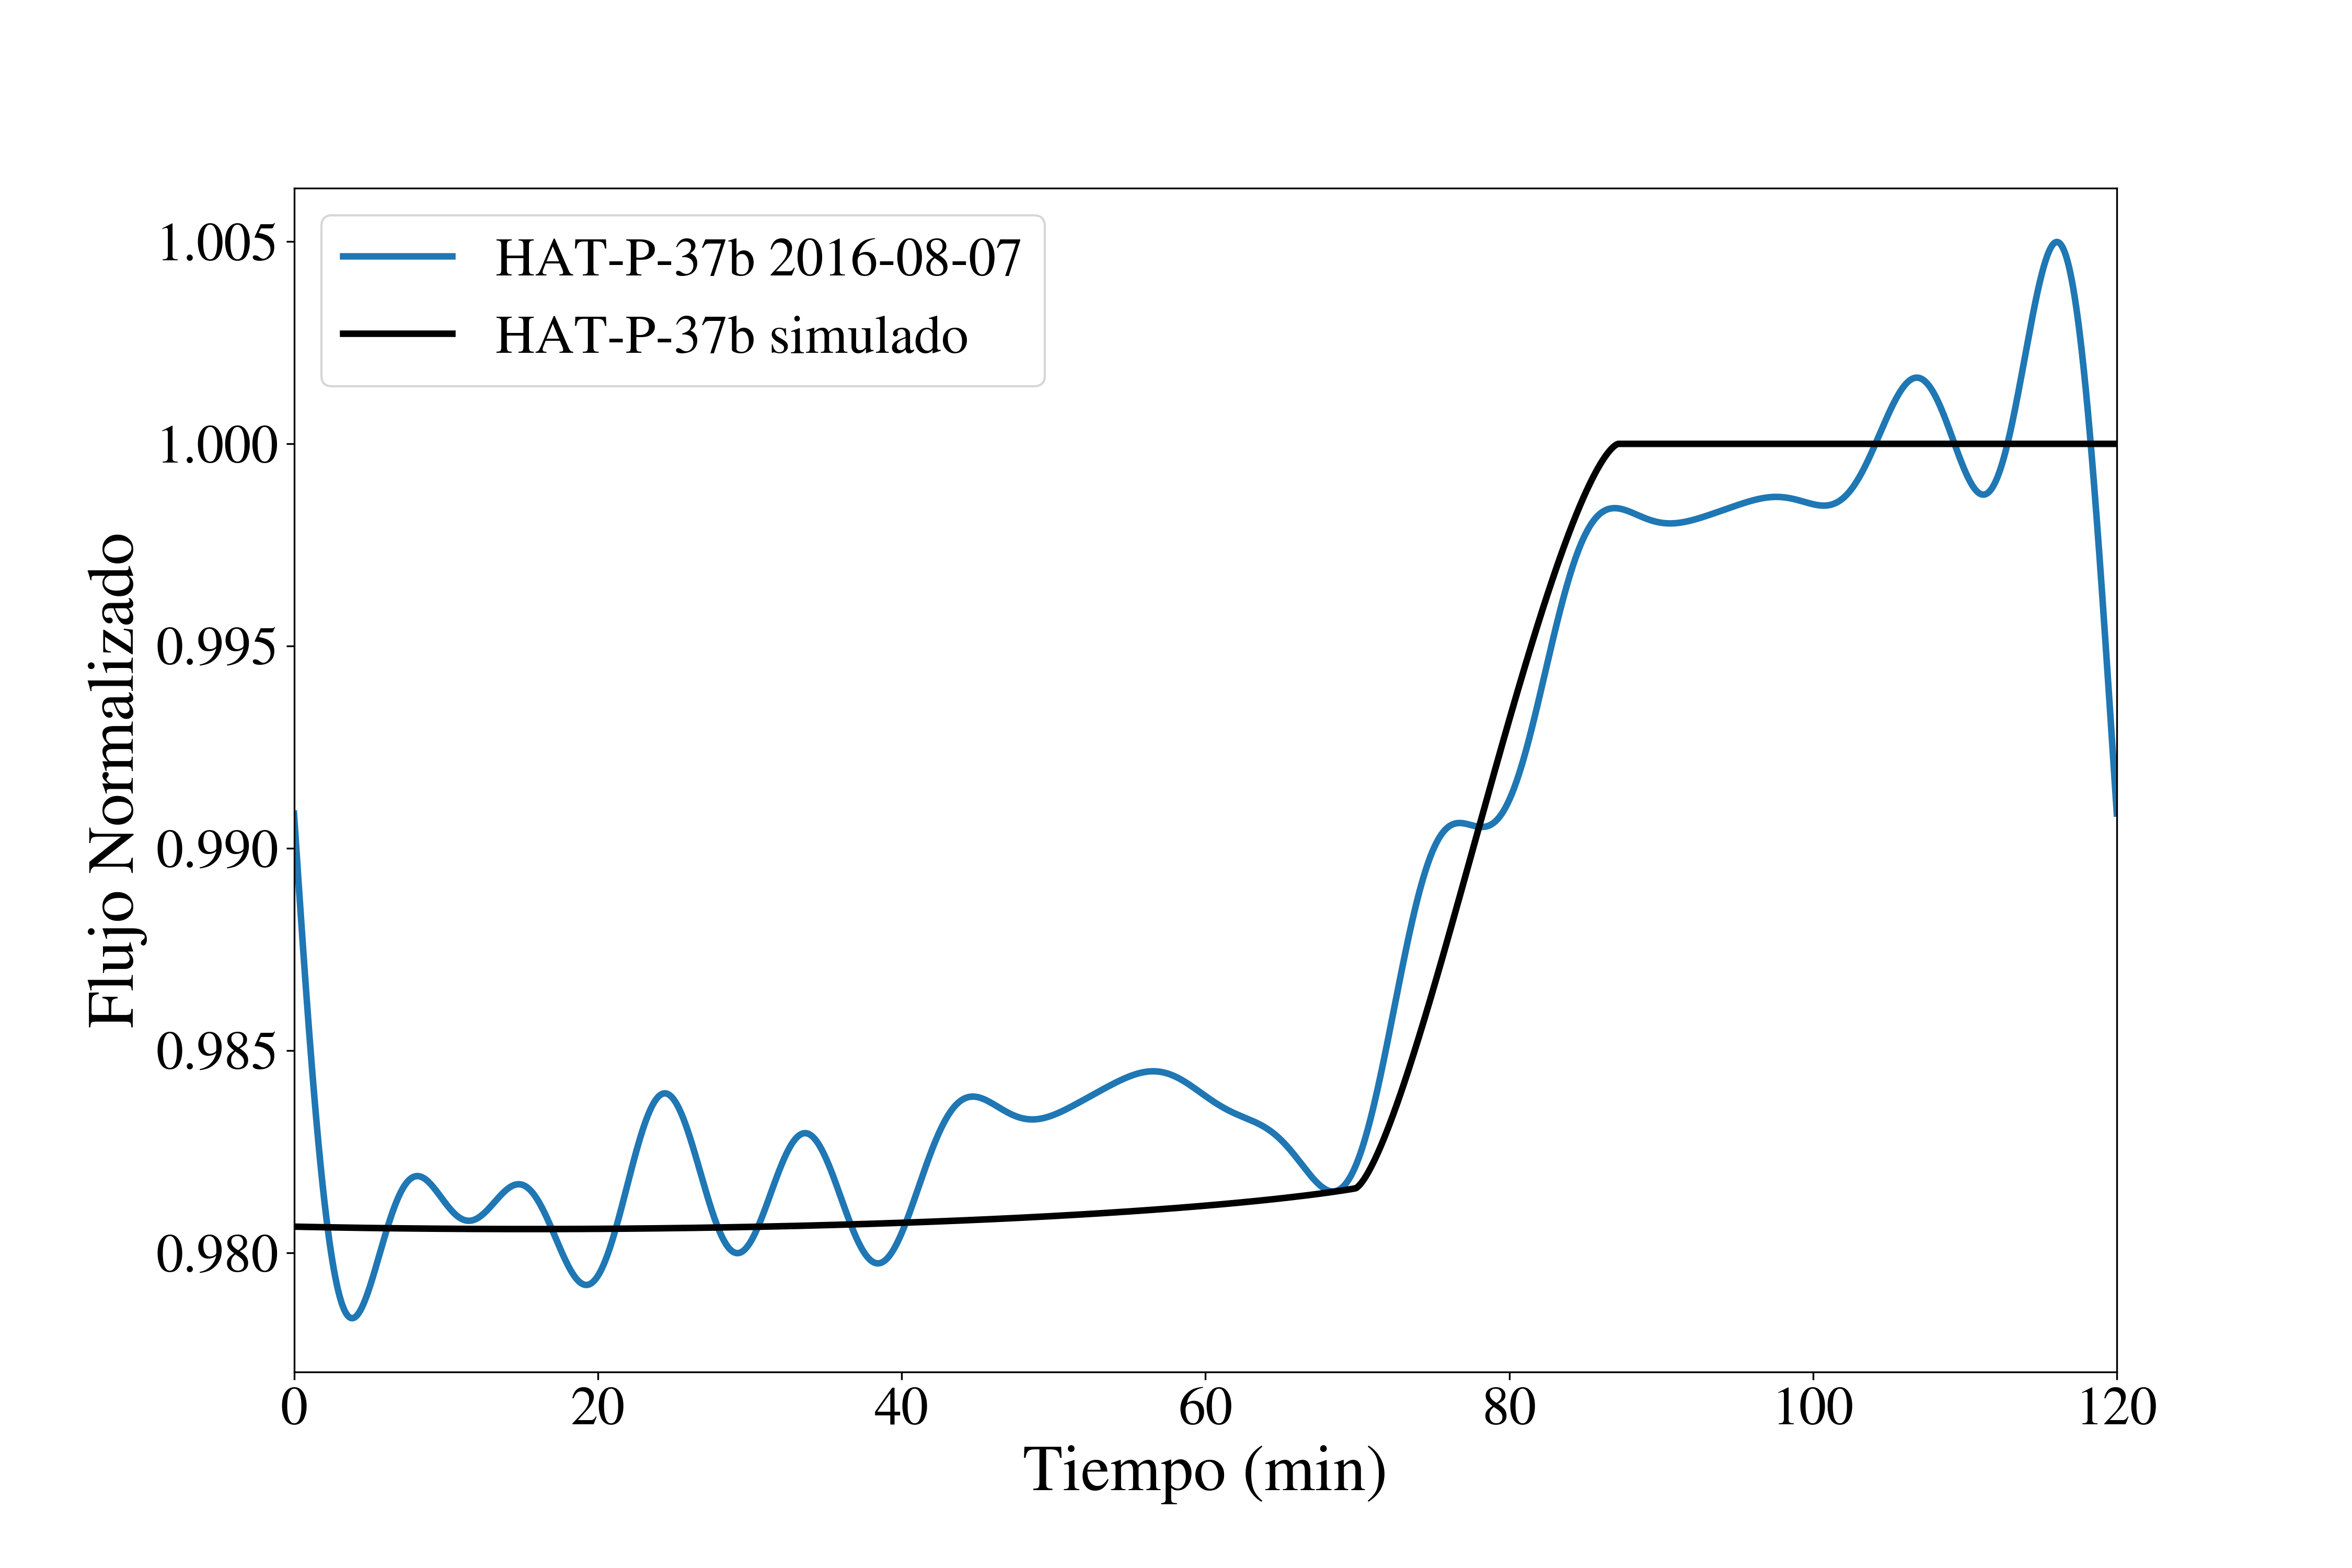
\includegraphics[max size={0.9\textwidth}{0.9\textheight}]{./figures/hat37b_fou_2.png}
	 \caption{Azul: curva de luz de HAT-P-37b después del filtrado de altas frecuencias. La señal a ruido resultante fue de $SNR=124.75$. La línea negra representa el modelo teórico, utilizando los parámetros presentados en \cite{bakos2012hat}. El coeficiente de correlación entre la curva y el modelo es $C=0.982$.}
	  \label{fig_transito_fou}
  \end{figure}

\subsubsection*{IV.2.1.2 Resultados del promedio móvil}
\addcontentsline{toc}{subsubsection}{IV.2.1.2 Resultados del promedio móvil}

En la figura \ref{fig_transito_mov} podemos apreciar el resultado del promedio móvil, aplicado a la curva de luz de HAT-P-37b. Para este resultado, se utilizó una ventana de 3000 frames. De igual manera se muestra en negro el modelo teórico. La similitud entre el modelo y la curva filtrada es alto, el coeficiente de correlación es de $C=0.962$.

\begin{figure}[h!]
\centering
	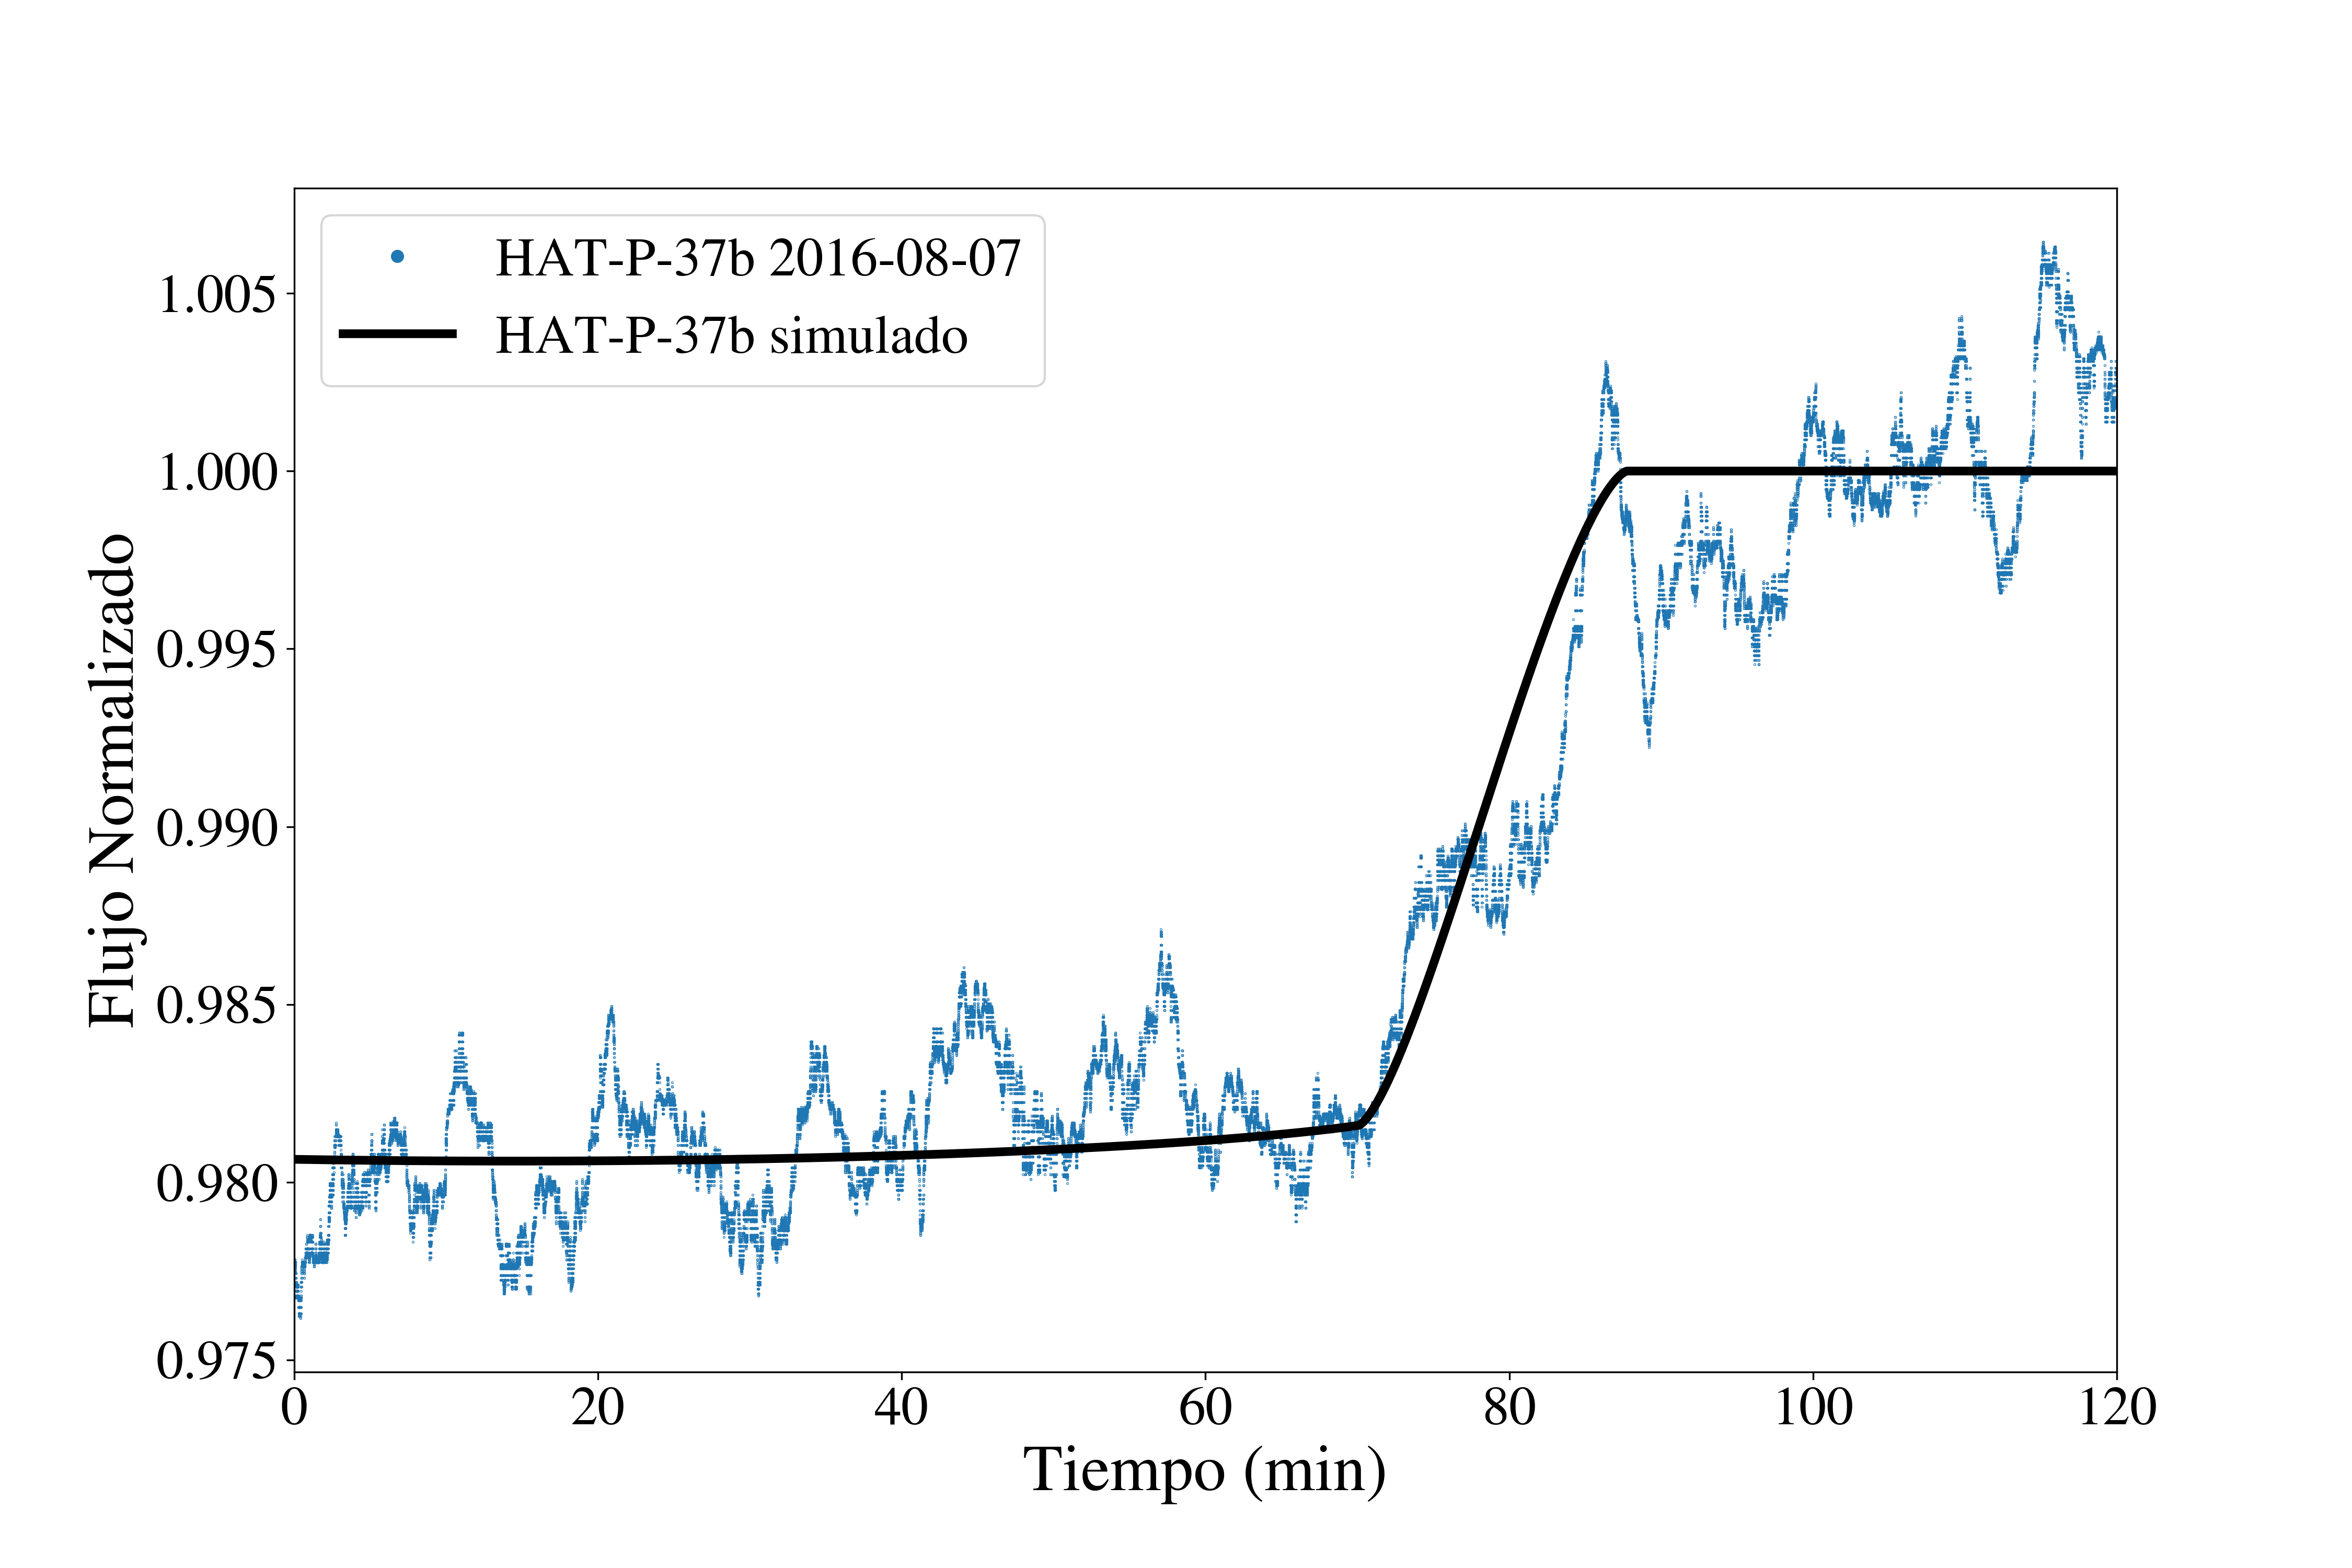
\includegraphics[max size={0.9\textwidth}{0.9\textheight}]{./figures/hat37b_mov_2.png}
	\caption{Azul: curva de luz de HAT-P-37b después del promedio móvil. La señal a ruido resultante fue de $SNR=116.64$. La línea negra representa el modelo teórico, utilizando los parámetros presentados en \cite{bakos2012hat}. El coeficiente de correlación entre la curva y el modelo es $C=0.962$.}
	\label{fig_transito_mov}
\end{figure}

Como se observa en la figura \ref{fig_transito_mov}, este método altera la pendiente de la curva, donde el planeta está saliendo de la superficie solar. Esta deformación es proporcional a la longitud de la ventana de promediado, por lo que ventanas pequeñas (1000-3000 frames) pueden dar mejores coeficientes de correlación. 


\subsubsection*{IV.2.1.3 Resultados de PCA}
\addcontentsline{toc}{subsubsection}{IV.2.1.3 Resultados del PCA}

En la figura \ref{fig_transito_pca} podemos apreciar el resultado del filtrado utilizando el análisis de componentes principales (PCA), aplicado a la curva de luz de HAT-P-37b. Se calcularon las componentes principales de un conjunto de 25 tránsitos simulados con diferentes $\Delta F$ y $t_{c}$. Debido a que la componentes principales son calculadas utilizando una variedad de parámetros, la curva resultado solo posee la forma de tránsito, sin embargo, no es ideal para ser utilizada para el cálculo de observables.

\begin{figure}[h!]
	\centering
		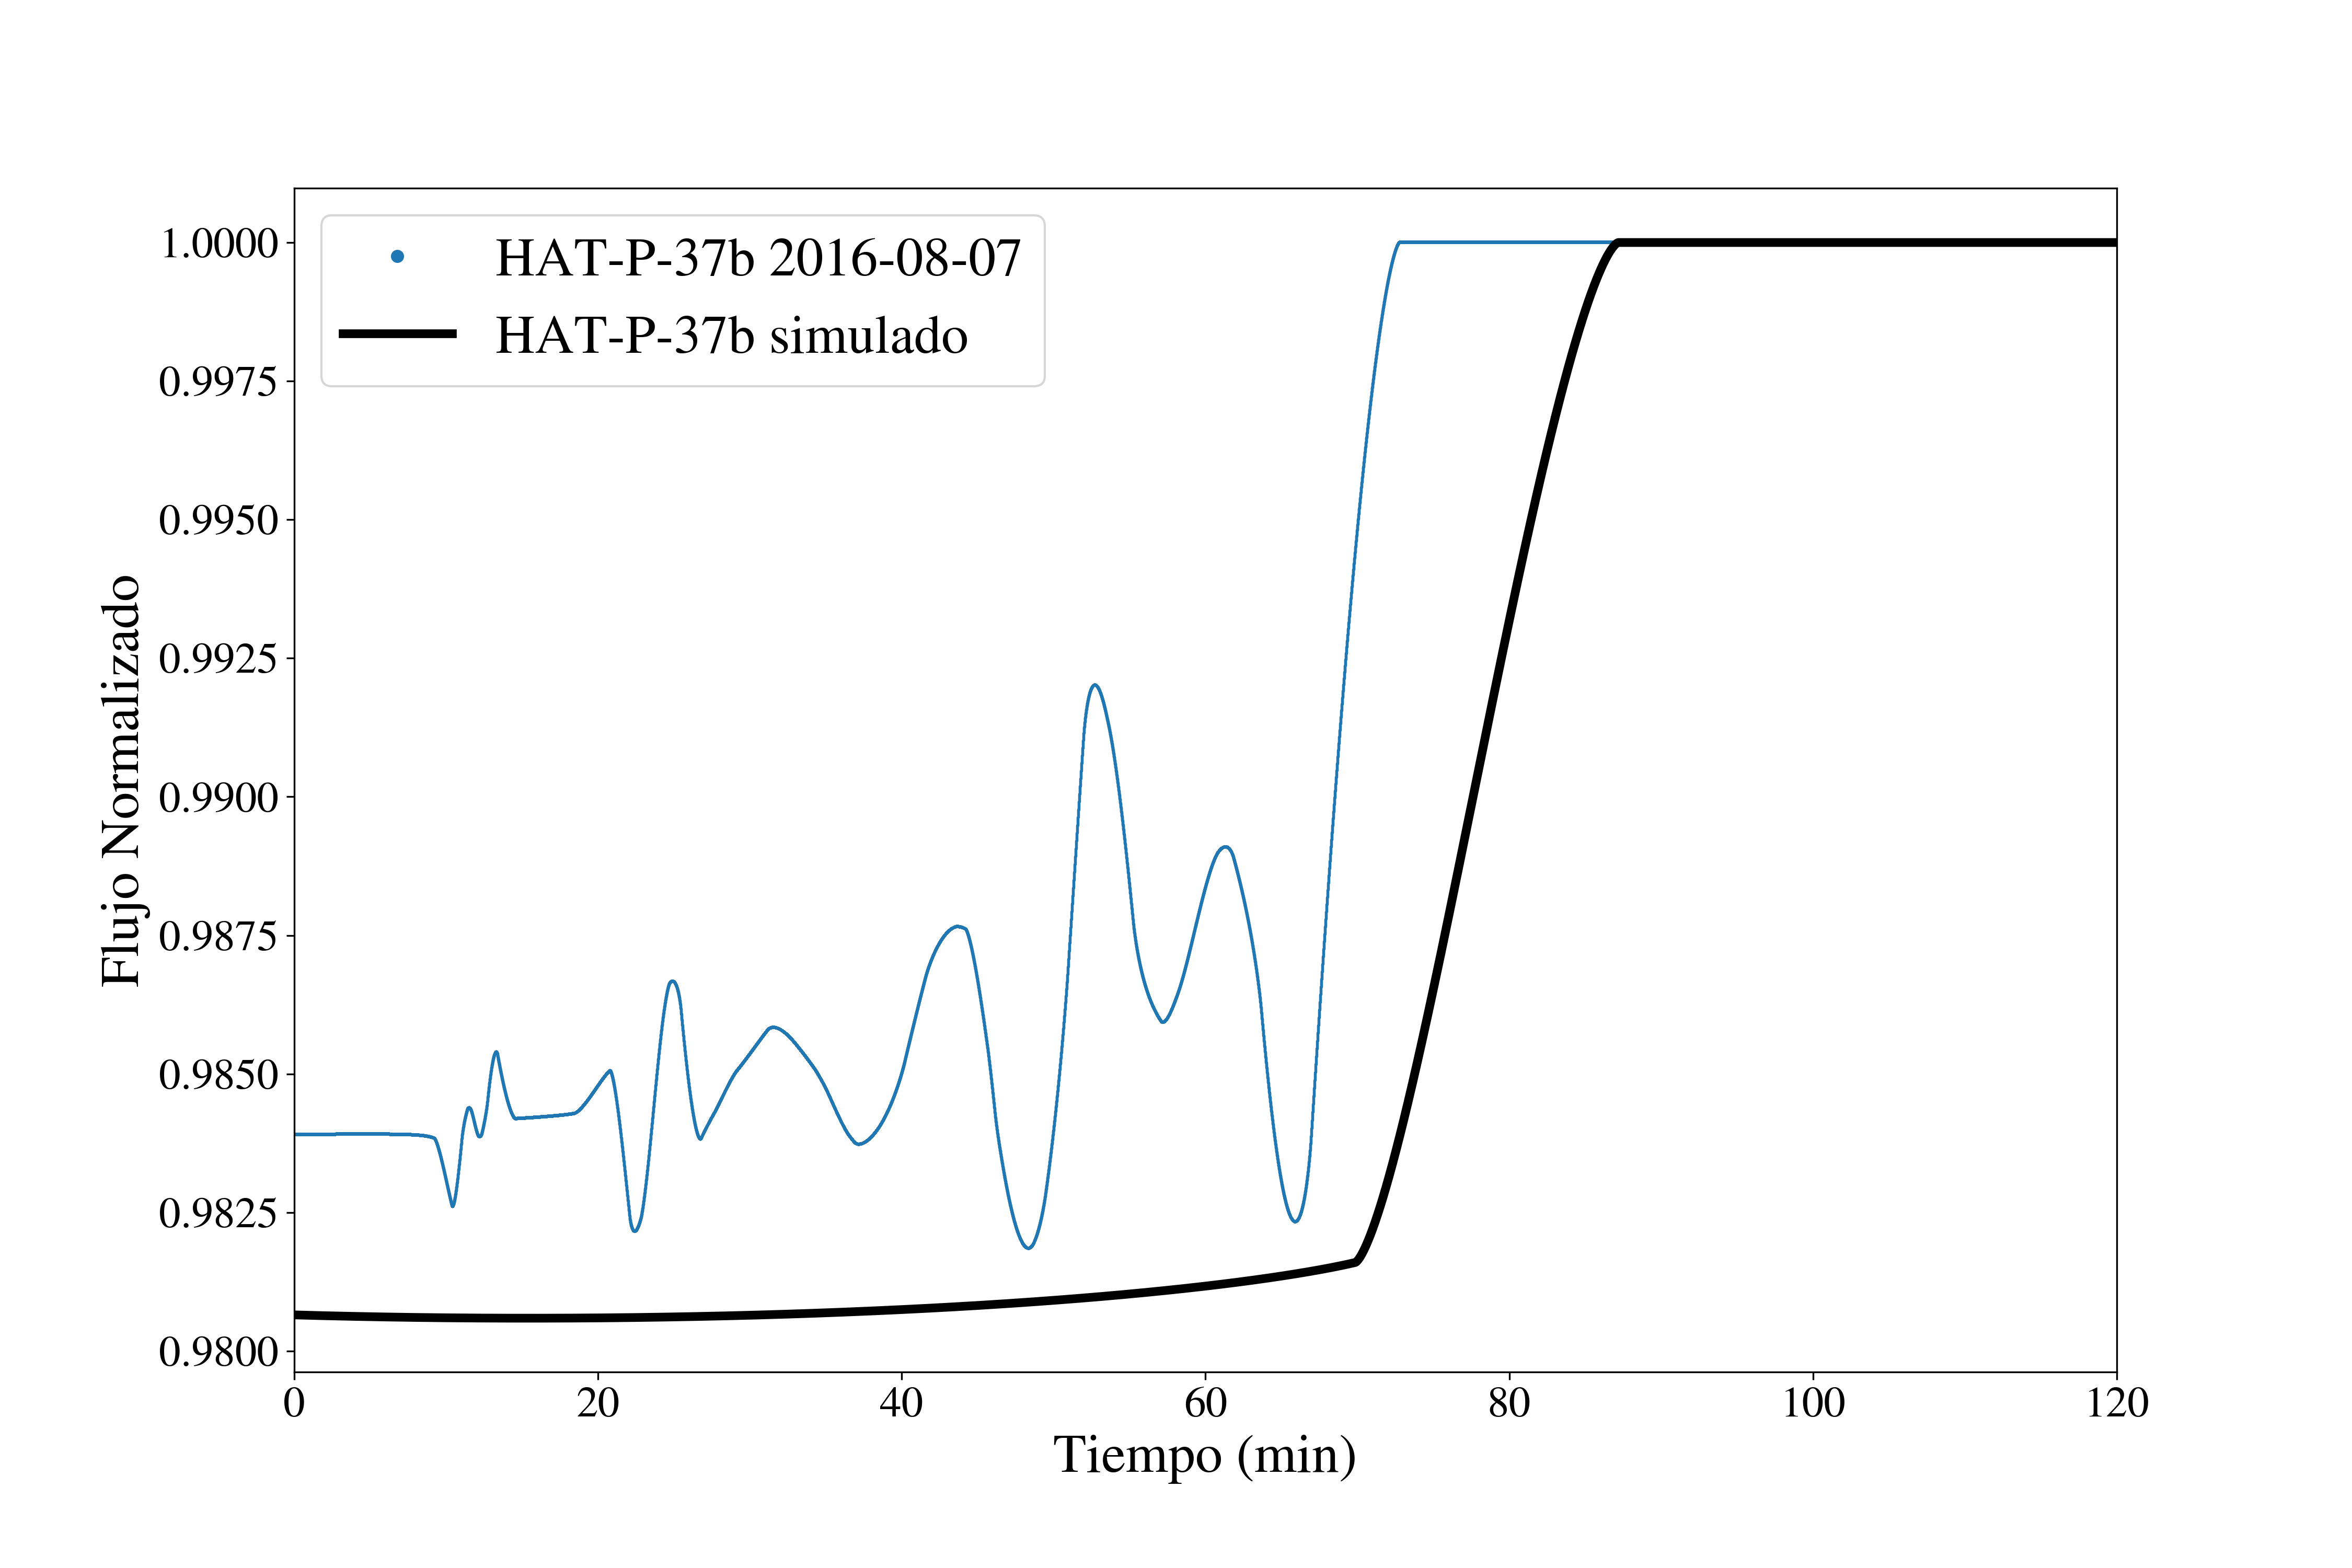
\includegraphics[max size={0.9\textwidth}{0.9\textheight}]{./figures/hat37b_pca_2.png}
		\caption{Azul: curva de luz de HAT-P-37b después del filtrado con PCA. La señal a ruido resultante fue de $SNR=135.51$. La línea negra representa el modelo teórico, utilizando los parámetros presentados en \cite{bakos2012hat}. El coeficiente de correlación entre la curva y el modelo es $C=0.889$.}
		\label{fig_transito_pca}
\end{figure}

Esta metodología funciona para la visualización, y como método de comparación entre los modelos teóricos y las curvas de luz. Si las curva de luz, contiene componentes principales similares a las del modelo, se producirá una curva similar a la que se observa en la figura \ref{fig_transito_pca}. Si la curva es solo ruido, el resultado será una curva errática sin ningún parecido con el modelo.\textcolor{red}{HAY QUE PRESENTAR UN EJEMPLO DE ESTO}


\subsubsection*{IV.2.1.4 Resumen de resultados con datos observacionales}
\addcontentsline{toc}{subsubsection}{IV.2.1.4 Resumen de resultados con datos observacionales}

En la tabla \ref{tab_resultados_obs} se presentan todos los resultados de la mejora de la SNR utilizando las metodologías descritas anteriormente, para todo el conjunto de curvas de luz reales (véase III.1)

\begin{table}
	\centering
	\begin{footnotesize}
	\begin{tabular}{ccccccccc}
	\hline 
	Fecha & Nombre & SNR & $\mbox{SNR}_{Fourier}$ &  $\mbox{SNR}_{mov}$ & $\mbox{SNR}_{PCA}$\\ 
	\hline
	06/Ago/2016 & WASP74b$^{1}$ & 47.03 & 226.50 & 212.93 & 279.51 \\ 
	06/Ago/2016 & WASP74b$^{2}$ & 39.82 & 114.47 & 114.73 & 156.30 \\
	06/Ago/2016 & HAT-P-32b & 14.55 & 29.68 & 29.43 & 31.85 \\
	07/Ago/2016 & HAT-P-37$^{1}$ & 11.66 & 176.44 & 166.00 & 180.11 \\ 
	07/Ago/2016 & HAT-P-37$^{2}$ & 11.73 & 124.75 & 116.64 & 135.51 \\ 
	28/May/2017 & HAT-P-14b & 61.40 & 154.80 & 158.96 & - \\ 
	29/May/2017 & WASP74b & 9.46 & 93.33 & 82.86 & 93.86 \\
	31/May/2017 & WASP48b & 7.74 & 61.25 & 48.16 & 63.29 \\  
	31/May/2017 & WASP74b & 14.70 & 41.36 & 42.60 & 47.97 \\
	02/Jun/2017 & WASP-48b$^{1}$ & 11.07 & 28.10 & 22.91 & 32.71 \\
	02/Jun/2017 & WASP48b$^{2}$ & 7.67 & 20.37 & 14.78 & 20.32 \\
	05/Jun/2017 & HAT-P-31b & 6.17 & 68.05 & 43.67 & 80.09 \\
	08/Jun/2018 & Kepler17b & 146.52 & 523.31 & 512.25 & 602.00 \\ 
	\hline 
	\end{tabular} 
	\end{footnotesize}
	\caption{Resumen de los resultados para mejorar la SNR en las curvas de luz de tránsitos de exoplanetas obtenidas en múltiples temporadas en el OAN-SPM. SNR indica el valor de ruido después de la fotometría. $\mbox{SNR}_{Fourier}$, $\mbox{SNR}_{mov}$ y $\mbox{SNR}_{PCA}$ indican el valor de ruido resultado del filtrado de Fourier, promedio móvil y PCA respectivamente. Los superíndices indican que la misma curva se dividió en 2 segmentos de 2 horas cada uno, los cuales se analizaron de manera independiente.}
	\label{tab_resultados_obs}
	\end{table}

Todas las curvas de luz de la tabla \ref{tab_resultados_obs} tienen una duración de 2 horas y fueron obtenidas al momento del tránsito de exoplanetario. En la mayoría de las ocasiones, solo se observó la entrada o salida del exoplaneta al disco solar, las curvas con el superíndices ($^{1,2}$) indican que se observó el tránsito completo y se separó en segmentos de 2 horas para su análisis, donde ($^{1}$ y $^{2}$) indican el comienzo y el final del tránsito respectivamente.

\subsection*{IV.2.2 Determinación de candidatos a tránsitos}
\addcontentsline{toc}{subsection}{IV.2.2 Determinación de candidatos a tránsitos}

Cabe destacar que las técnicas de filtrado utilizadas para la mejora de la SNR, deforman la curva de luz, por lo que no es posible recuperar la curva exacta del tránsito. Sin embargo, el objetivo es encontrar variaciones en el flujo, para determinar si la estrella observada puede ser candidata a tener un exoplaneta.

Se aplicó un ajuste del modelo trapezoidal (véase III.6.1) a las curvas filtradas. El desempeño de los distintos método de filtado, se evaluó utilizando el valor de $\Delta F$ resultado del ajuste a los datos filtrados y comparándolo con el valor reportado por la comunidad en bases de datos como \href{http://var2.astro.cz/ETD/index.php}{\textit{Exoplanet Transit Database}}. Estos resultados se aprecian en la tabla \ref{tab_resultados_profundidad}.


\begin{table}
	\centering
	\begin{tabular}{ccccccccc}
	\hline 
	Fecha & Nombre & $\Delta F$ (\%) & $\Delta F_{Fourier}$ (\%) &  $\Delta F_{mov}$ (\%) & $\Delta F_{PCA}$ (\%) \\ 
	\hline
	06/Ago/2016 & WASP74b$^{1}$ & 1.04 & - & - & - \\ 
	06/Ago/2016 & WASP74b$^{2}$ & 1.04 & - & - & - \\
	06/Ago/2016 & HAT-P-32b$^{1}$ & 2.44 & - & - & - \\
	07/Ago/2016 & HAT-P-37$^{1}$ & 2.04 & 1.63 & 1.67 & 1.75 \\ 
	07/Ago/2016 & HAT-P-37$^{2}$ & 2.04 & 1.74 & 1.84 & 1.91 \\ 
	28/May/2017 & HAT-P-14b$^{1}$ & 0.5 & - & - & - \\ 
	29/May/2017 & WASP74b$^{2}$ & 1.04 & 2.42 & 2.59 & 1.62 \\ 
	31/May/2017 & WASP48b$^{2}$ & 1.0 & - & - & - \\  
	31/May/2017 & WASP74b$^{1}$ & 1.04 & 6.47 & 6.28 & 6.59 \\
	02/Jun/2017 & WASP-48b$^{1}$ & 1.0 & 6.63 & 5.33 & 7.5 \\
	02/Jun/2017 & WASP48b$^{2}$ & 1.0 & - & - & - \\
	05/Jun/2017 & HAT-P-31b$^{1}$ & 1.23 & - & - & - \\
	08/Jun/2018 & Kepler17b$^{1}$ & 2.13 & - & - & - \\ 
	\hline 
	\end{tabular} 
	\caption{Resultados de $\Delta F$ obtenidos ajustando el modelo del trapezoide a las curvas de luz de tránsitos. $\Delta F_{Fourier}$, $\Delta F_{mov}$ y $\Delta F_{PCA}$ representan el valor de $\Delta F$ obtenido después del filtrado de Fourier, promedio móvil y PCA respectivamente. El superíndice $^{1}$ indica que a curva de luz fue obtenida mediante el inicio del tránsito y $^{2}$ indica que la curva contenía el final del tránsito.}
	\label{tab_resultados_profundidad}
	\end{table}

El ajuste trapezoidal, nos regresa como resultado dos parámetros, $\Delta F$ y $t_{c}$ (véase II.1.1). En estos resultados evaluamos solamente el valor de $\Delta F$, esto nos brinda información sobre la magnitud del cambio en el flujo de la estrella observada, el cual es uno de los principales criterios para la selección de un posible candidato a tránsito. 

Los signos (-) en la tabla \ref{tab_resultados_profundidad}, indican que el método de ajuste falló. Esto ocurre cuando el ajuste del modelo nos da como resultado un valor de $\Delta F$ fuera de los límites permitidos. En este estudio fijamos los límites de $\Delta F$ como 0.2\%-5\%, y para $t_{c}$ como 15-60 minutos, siendo estos los límites inferior y superior respectivamente. Esto nos indica que la detectabilidad fue baja (38\%), en la mayoría de los casos negativos, las curvas de luz tenían tendencias de baja frecuencia después del proceso de fotometría.